% =============================================================================
% Hessian Spectra During Grokking
% Flavio Gualtieri
%
% Working draft. Every number below is taken from a file generated by a script
% in this repository; the source is named in a comment next to it:
%   reports/sweep_summary.md                         python scripts/sweep_summary.py
%   reports/figures/gate_p91_wd{0.6,1}_seed0_summary.md
%                                                    python -m eigengrok.analysis.make_figures
%   reports/figures/effective_rank_multiseed_summary.md
%                                                    python -m eigengrok.analysis.aggregate_effective_rank
%   reports/hessian_validation.md                    python scripts/validate_hessian_real.py
%   reports/spectral_validation.md                   (historical; previous estimator)
% Figures are read from reports/figures/ (see README for the commands).
%
% TODO(Phase 4): restructure into the workshop paper (intro, related work,
% setup, estimator validation, milestones and stability, forecasting
% results, limitations), with numbers pulled from a generated numbers.tex.
% Sections "Spectral observables" and "Estimator validation" still describe
% the previous estimator (eigenthings.py, last present at commit 9bf5fbe),
% which produced the spectra in reports/spectra/; the current one is
% eigengrok/hessian/.
% =============================================================================

\documentclass[11pt,a4paper]{article}

\usepackage[margin=2.0cm]{geometry}
\usepackage{mathpazo}
\usepackage{microtype}

\usepackage{amsmath}
\usepackage{amssymb}
\usepackage{amsthm}

\usepackage{graphicx}
\graphicspath{{../reports/figures/}}
\usepackage{booktabs}
\usepackage{enumitem}
\usepackage[font=small,labelfont=bf,skip=4pt]{caption}
\usepackage{subcaption}
\usepackage{titlesec}
\titlespacing*{\section}{0pt}{1.0ex plus .2ex}{0.5ex plus .1ex}
\titlespacing*{\subsection}{0pt}{0.9ex plus .2ex}{0.4ex plus .1ex}
\titlespacing*{\paragraph}{0pt}{0.6ex plus .1ex}{1em}
\setlength{\tabcolsep}{5pt}
\renewcommand{\arraystretch}{1.0}
\setlength{\abovedisplayskip}{5pt}
\setlength{\belowdisplayskip}{5pt}
\setlength{\abovedisplayshortskip}{3pt}
\setlength{\belowdisplayshortskip}{3pt}

\usepackage{natbib}
\usepackage[hidelinks]{hyperref}
\raggedbottom
\renewcommand{\textfraction}{0.05}
\renewcommand{\topfraction}{0.95}
\renewcommand{\bottomfraction}{0.95}
\renewcommand{\floatpagefraction}{0.85}

% ----------------------------------------------------------------------------
% Macros
% ----------------------------------------------------------------------------
\newcommand{\R}{\mathbb{R}}
\newcommand{\bH}{\mathbf{H}}

% Visible placeholder box for figures that are not yet produced
\newcommand{\figtodo}[1]{\par\vspace{4pt}\noindent\fbox{\parbox{0.97\linewidth}%
  {\footnotesize\textbf{TODO (figure):} #1}}\par\vspace{4pt}}

% ----------------------------------------------------------------------------
\title{Hessian Spectra During Grokking}
\author{Flavio Gualtieri}
\date{\today}

\begin{document}
\maketitle

% #############################################################################
\section{Grokking and motivation}
\label{sec:hess-intro}
% #############################################################################

Grokking was first reported by \citet{power2022grokking}. It is a phenomenon by which a model attains near-perfect training
accuracy quickly, then remains at chance-level test accuracy for an extended period,
and then transitions sharply to high test accuracy long after the training loss has saturated.  This delay is the object of interest: whatever separates the memorizing phase from the generalizing one is not directly visible in the training loss, which suggests studying the local geometry of the loss landscape to understand the transition. This note uses the Hessian's eigenvalue spectrum as
a description of this geometry, following \citet{fort2018goldilocks}, and
estimates it by the Lanczos-based approach of \citet{yao2020pyhessian}, which
recovers spectral information without explicitly forming the Hessian, a gigantic object for anything beyond a low-parameter toy model. The approximation machinery is implemented directly (Section~\ref{sec:hess-lanczos}) rather than through the PyHessian library.

The setting is modular arithmetic, which the literature -- \citet{gromov2023grokking} in particular -- treats as the natural context for this problem.
The experiments use modular addition ($a + b \bmod p$) with a small
decoder-only transformer trained with AdamW and weight decay large enough to
penalize the pure-memorization solution. Training accuracy reaches 99\% within a few thousand optimization steps
% source: reports/sweep_summary.md (pooled median t_mem; Section "Init scale")
(pooled median $200$ steps at initialization scale $\alpha=1$, $2{,}000$ at $\alpha=8$),
while test accuracy stays near chance ($1/p$) for several thousand further steps
% source: reports/sweep_summary.md (pooled median gap t_onset - t_mem)
(median gap to the first test accuracy $\ge 0.5$: $4{,}800$ steps at $\alpha=1$, $4{,}000$ at $\alpha=8$)
before rising above 95\% (Figure~\ref{fig:hess-wd-curve}). The length of that delay, and its
dependence on weight decay and initialization scale, is the phenomenon this note addresses.

\begin{figure}[ht]
\centering
\figtodo{Train and test accuracy vs.\ optimization step (log scale), $p=91$, wd$=0.5$, $\alpha=1$, mean $\pm$ std over the 10 seeds, from \texttt{reports/wd\_sweep\_accuracy\_curves.csv}. No script in the repository generates this figure yet.}
\caption{Train and test accuracy vs.\ optimization step for the modular-addition task, establishing the qualitative shape of the phenomenon before any spectral quantity is introduced.}
\label{fig:hess-wd-curve}
\end{figure}

% #############################################################################
\section{Spectral observables}
\label{sec:hess-observables}
% #############################################################################

For network parameters $\theta \in \R^n$ and loss function $\mathcal{L}(\theta)$, the Hessian is
$\bH = \nabla^2_\theta \mathcal{L}(\theta) \in \R^{n\times n}$, symmetric with
eigenvalues $\lambda_1 \le \cdots \le \lambda_n$. Rather than individual eigenvalues, eight scalar summaries of the full spectrum are tracked at a series of checkpoints:

\begin{enumerate}[leftmargin=*,itemsep=1pt,label=(\roman*)]
    \item \texttt{top\_eig}: the largest eigenvalue $\lambda_n$.
    \item \texttt{bulk\_edge}: a robust threshold separating the bulk of the
    spectrum from its outliers.
    \item \texttt{n\_outliers}: the number of eigenvalues above
    \texttt{bulk\_edge}.
    \item \texttt{trace}: $\mathrm{tr}\,\bH = \sum_i \lambda_i$.
    \item \texttt{spectral\_entropy}: the Shannon entropy of the normalised
    spectral measure.
    \item \texttt{effective\_rank}: the exponential of \texttt{spectral\_entropy}.
    \item \texttt{negative\_mass}: the spectral mass on meaningfully negative
    eigenvalues.
    \item \texttt{conditioning}: the ratio \texttt{top\_eig}/\texttt{bulk\_edge}.
\end{enumerate}

% #############################################################################
\section{Spectral estimation}
\label{sec:hess-lanczos}
% #############################################################################

For a network with a number of parameters in the $10^3$--$10^7$ range, forming
$\bH$ explicitly is infeasible, so the observables above are estimated with
stochastic Lanczos quadrature. Writing
$g(\theta) = \nabla_\theta \mathcal{L}(\theta)$, and given a Krylov depth $m$
and probe count $k$, the procedure is:

\begin{enumerate}[leftmargin=*,itemsep=1pt]
    \item \textbf{Hessian--vector products.} Pearlmutter's identity gives
    $\bH v = \nabla_\theta\!\left(g(\theta)^\top v\right)$ from two backward
    passes, so $\bH$ is only ever accessed through the map $v \mapsto \bH v$.
    \item \textbf{Lanczos.} For each probe $j = 1,\dots,k$: draw a random unit
    vector $v^{(j)}$ and run $m$ steps of the Lanczos recurrence, calling
    step~1 once per step, to obtain a tridiagonal
    $T^{(j)} \in \R^{m \times m}$ --- the projection of $\bH$ onto the order-$m$
    Krylov subspace generated by $v^{(j)}$.
    \item \textbf{Quadrature rule.} Eigendecompose
    $T^{(j)} = U^{(j)} \Lambda^{(j)} U^{(j)\top}$. The Ritz values
    $\lambda_i^{(j)} = \Lambda^{(j)}_{ii}$ are the quadrature nodes and
    $w_i^{(j)} = \big(U^{(j)}_{1i}\big)^2$ the weights; this rule matches the
    first $2m-1$ moments of the spectral measure of $\bH$ seen by $v^{(j)}$.
    \item \textbf{Pooling.} Average over probes,
    $\hat\mu = \frac{1}{k}\sum_{j=1}^{k}\sum_{i=1}^{m} w_i^{(j)}\,
    \delta_{\lambda_i^{(j)}}$, giving an estimate of the full spectral measure.
    \item \textbf{Observables.} Every quantity of
    Section~\ref{sec:hess-observables} is a functional of $\hat\mu$; for
    instance $\widehat{\mathrm{tr}}\,\bH = n\!\int\!\lambda \, d\hat\mu$.
\end{enumerate}

The Krylov depth $m$ and probe count $k$ are the two parameters trading compute
against accuracy.

% #############################################################################
\section{Estimator validation}
\label{sec:hess-validation}
% #############################################################################

All eight observables were validated against two exact-reference fixtures with
known ground-truth spectra: a small MLP whose Hessian can be materialized in full, and a quadratic form with a chosen spectrum. The validation identified two estimator
defects, distinct from mere under-convergence. First, the original
\texttt{bulk\_edge} and \texttt{conditioning} definitions used an unweighted
median and MAD over the Ritz values, which was biased by 30--50\% at every
Krylov depth: Lanczos node placement is moment-matching rather than
density-matching, so an unweighted median over-trusts the sparse nodes near the
spectral edge. Second, the original \texttt{negative\_mass} definition
integrated mass immediately either side of the zero crossing and therefore
measured Lanczos noise rather than curvature; it is now margin-thresholded. Both
were corrected. Table~\ref{tab:hess-mk} reports the resulting
per-observable convergence requirements.

\begin{table}[htbp]
\centering
\small
\begin{tabular}{lccc}
\toprule
Observable & Governed by & Minimum $m$ & Minimum $k$ \\
\midrule
trace & $k$ (Monte Carlo, $\propto k^{-1/2}$) & irrelevant & $\ge 100$ \\
top\_eig & $m$ & $\ge 20$ & $1$ \\
negative\_mass (margin-thresholded) & $m$ & $\ge 30$--$50$ & $\ge 30$ \\
spectral\_entropy / effective\_rank & $m$ & $\ge 20$--$30$ & $\ge 30$ \\
bulk\_edge / conditioning (post-fix) & $m$ & $\ge 75$--$100$ & not yet swept \\
\bottomrule
\end{tabular}
\caption{Approximation accuracy against Lanczos depth $m$ and probe count $k$,
measured on the exact-reference fixtures
(\texttt{reports/spectral\_validation.md}). The spectra in
\texttt{reports/spectra/} were computed with $m=100$, $k=100$ on a fixed
512-example batch of the training set.}
\label{tab:hess-mk}
\end{table}

The fixtures above have roughly $10^3$ parameters. The current estimator
(\texttt{eigengrok/hessian/}) has since also been checked on a trained
modular-addition network: \texttt{reports/hessian\_validation.md} compares
several $(m, k)$ settings against a high-accuracy reference ($m=150$, $k=128$)
on 25 checkpoints of the $p=91$, wd$=1$, seed~0 run, with the Hessian of the loss
on the full training set (2{,}484 examples).

% #############################################################################
\section{Experiments}
\label{sec:hess-experiments}
% #############################################################################

All current experiments run on modular addition with a small decoder-only
transformer on $a+b \bmod p$, and this setting is the source of every measured
number reported below. Two hyperparameters control the onset of grokking on this
task, and both were
swept with logged runs (AdamW with PyTorch's default $\beta = (0.9, 0.999)$, full-batch, $p=91$, training fraction $0.3$, $150{,}000$
steps). Weight decay was swept from $0.45$ to $1.0$ in steps of $0.05$, ten
seeds per setting. Initialization scale was swept at $\alpha \in \{1,8\}$, where
every parameter is multiplied by the scalar $\alpha$ after standard
initialization. Onset is the first logged step with test accuracy $\ge 0.5$;
intervals are 95\% bootstrap intervals over seeds (definitions and every number
in this section: \texttt{reports/sweep\_summary.md}).

% source: reports/sweep_summary.md, Sections "Weight decay" and "Means, final accuracy ..."
\paragraph{Weight decay.} Larger weight decay produces an earlier onset at both
initialization scales (Spearman correlation between weight decay and onset $-0.77$
at $\alpha=1$ and $-0.82$ at $\alpha=8$, 120 runs each), though not strictly
monotonically at $\alpha=8$ (Figure~\ref{fig:onset-wd}). At $\alpha=1$ the mean
onset falls from $8{,}660$ steps at wd$=0.45$ to $3{,}510$ at wd$=1.0$. Relative
to wd$=1.0$, wd$=0.45$ delays the mean onset by $2.47\times$ $[1.98, 3.04]$ at
$\alpha=1$ and $1.91\times$ $[1.31, 2.69]$ at $\alpha=8$; on medians the two
are close ($2.18\times$ $[1.73, 3.45]$ and $2.24\times$ $[1.81, 2.68]$), the
$\alpha=8$ mean at wd$=1.0$ being pulled up by a single late seed (onset at step
$14{,}800$, \texttt{reports/sweep\_milestones.csv}).

% source: reports/sweep_summary.md, Section "Init scale: init 8 against init 1 (baseline)"
\paragraph{Initialization scale.} Against $\alpha=1$ at the same weight decay,
$\alpha=8$ delays onset only moderately: the ratio of mean onsets ranges from
$1.07$ to $1.57$ across the 12 weight decays (median $1.22$), and its 95\%
interval excludes 1 at 6 of the 12. Pooled over weight decays, the
geometric-mean ratio is $1.21$ $[1.15, 1.28]$. What $\alpha=8$ mainly delays is
memorization: the pooled median first step with train accuracy $\ge 0.99$ is
$200$ at $\alpha=1$ and $2{,}000$ $[1{,}900, 2{,}000]$ at $\alpha=8$. The
memorization-to-onset gap is in fact shorter at $\alpha=8$ (pooled median
$4{,}000$ $[3{,}800, 4{,}250]$ against $4{,}800$ $[4{,}600, 5{,}100]$ steps,
ratio $0.83$ $[0.76, 0.89]$). An earlier version of this note reported that
$\alpha=8$ roughly doubles the onset delay; that figure came from the
first-crossing-of-twice-chance onset ($2{,}890$ against $1{,}350$ mean steps at
wd$=1.0$), a definition that several runs satisfy within the first few hundred
steps, long before the real transition, and it does not hold under the onset
definition used here.

% source: reports/sweep_summary.md, Section "Post-grokking collapses"
\paragraph{Instability after grokking.} Every run eventually holds test accuracy
$\ge 0.95$ for five consecutive evaluations, but none stays there: in every one
of the 240 runs test accuracy later falls from $\ge 0.95$ to $< 0.5$ and
recovers repeatedly, a median of 39 times per run (range 3--69), and training
accuracy collapses with it. These events are not yet diagnosed (TODO).

% #############################################################################
\section{Current results}
\label{sec:hess-status}
% #############################################################################

% source: reports/figures/gate_p91_wd{0.6,1}_seed0_summary.md, reports/figures/effective_rank_multiseed_summary.md
The Hessian spectrum has been computed from checkpoints of the
modular-addition sweep for 20 runs at $\alpha=1$: seeds 0--9 at wd$=0.6$ and at
wd$=1$ (\texttt{reports/spectra/}). Figure~\ref{fig:eff-rank} aligns the two
seed-0 runs on their own onset, here the first crossing of twice chance (step 3000
at wd$=0.6$ and 2400 at wd$=1$). In those two runs \texttt{effective\_rank}
falls by a similar factor after onset ($13.4\times$ and $14.2\times$) and
\texttt{top\_eig\_corr} rises ($2.7\times$ and $16.1\times$).

That agreement does not replicate across seeds. Over the ten seeds at each weight
decay the same collapse factor has mean $18.62\times$ (std $29.57$, range
$1.32$--$101.40\times$) at wd$=0.6$ and mean $41.32\times$ (std $30.33$, range
$4.52$--$86.46\times$) at wd$=1$. The factor is also measured from an onset
definition that is unreliable here: in 4 of the 10 seeds at each weight decay
the twice-chance crossing falls at or before step 300, thousands of steps
before test accuracy reaches 0.5, and at wd$=0.6$ the spectral window
(steps 100--6600 for seeds 1--9) ends before test accuracy reaches 0.5 in 4 of
the 10 seeds (\texttt{reports/sweep\_milestones.csv}).
\texttt{trace\_corr} disagrees in sign and timing between the two seed-0 runs and
does not survive an alternate-normalizer check
(\texttt{reports/figures/gate\_p91\_wd\{0.6,1\}\_seed0\_robustness.png}), so it
is not reported as a result. A further 5 of 66 checkpoints at wd$=0.6$ (19 of
150 at wd$=1$) of the seed-0 runs have a training-accuracy dip below 0.9 and are
flagged as unreliable (hollow markers in Figure~\ref{fig:eff-rank}).

\begin{figure}[ht]
\centering
\begin{subfigure}[t]{0.48\linewidth}
\centering
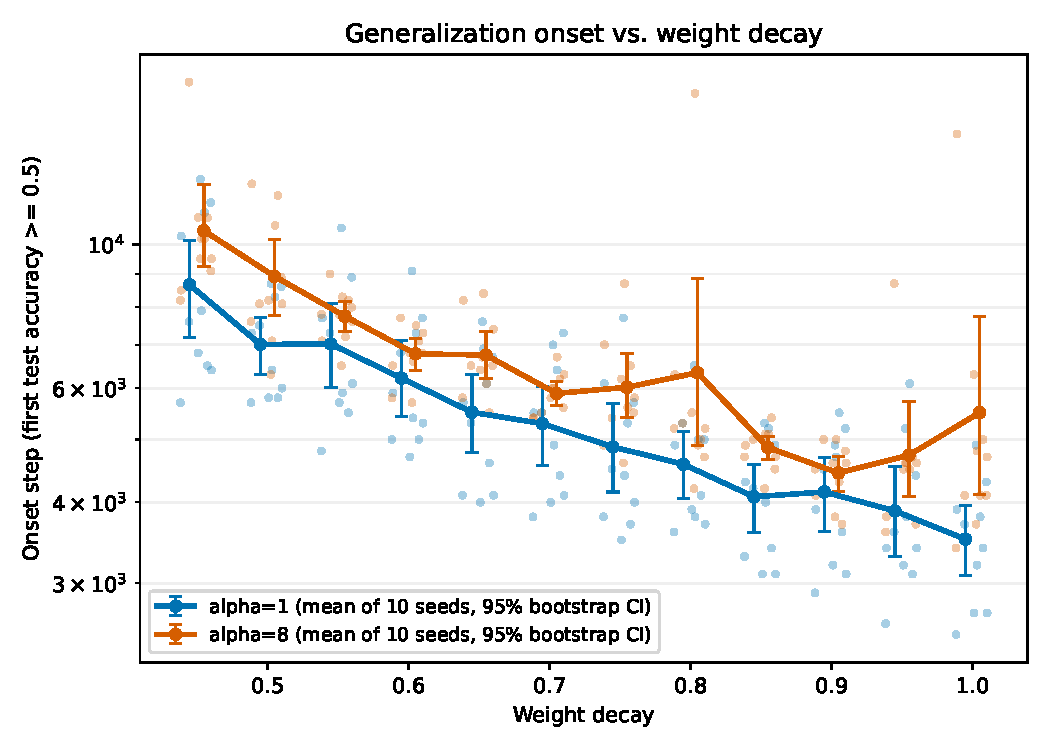
\includegraphics[width=\linewidth]{onset_vs_wd.pdf}
% source: reports/sweep_summary.md
\caption{Mean onset step (first test accuracy $\ge 0.5$) against weight decay for $\alpha=1$ and $\alpha=8$, with 95\% bootstrap intervals over the ten seeds per setting, each seed shown as a point. For $\alpha=1$, the mean onset falls from $8{,}660$ to $3{,}510$ steps as weight decay rises from 0.45 to 1.0. For $\alpha=8$ the decrease is noisier and not strictly monotone, and its mean onset sits above $\alpha=1$'s by a factor between $1.07$ and $1.57$ depending on weight decay, rather than a constant offset.}
\label{fig:onset-wd}
\end{subfigure}
\hfill
\begin{subfigure}[t]{0.48\linewidth}
\centering
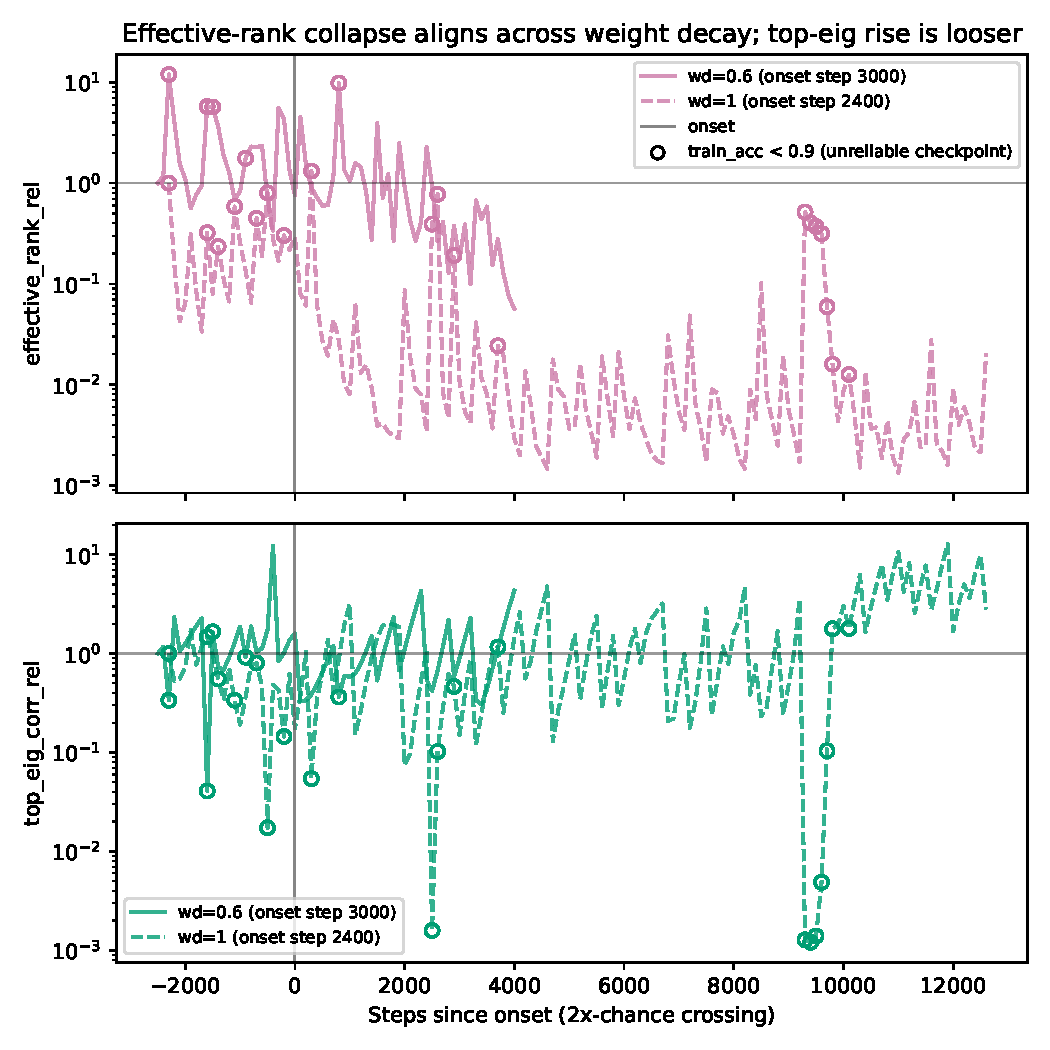
\includegraphics[width=\linewidth]{effective_rank_compare.pdf}
\caption{Effective rank (top) and top eigenvalue (bottom), both $\|\theta\|^{-2}$-corrected and normalized to a reference step, plotted against steps since each run's own twice-chance crossing (step 3000 at $wd=0.6$, step 2400 at $wd=1$), seed 0 only. Hollow markers flag checkpoints with training accuracy below 0.9 (5/66 at $wd=0.6$, 19/150 at $wd=1$). Effective rank falls by $13.4\times$ at $wd=0.6$ and $14.2\times$ at $wd=1$ after this onset and the top eigenvalue rises by $2.7\times$ and $16.1\times$; across ten seeds per weight decay the collapse factor varies by two orders of magnitude (see text), so the seed-0 agreement is not a stable effect. \texttt{trace\_corr} is omitted (see text).}
\label{fig:eff-rank}
\end{subfigure}
\caption{Weight decay controls grokking onset across the accuracy-only sweep
(a); the two seed-0 spectral runs of Section~\ref{sec:hess-status} (b) sit at
$wd=0.6$ and $wd=1$ within that same sweep.}
\label{fig:onset-eff-compare}
\end{figure}

% #############################################################################
\section{Next steps}
\label{sec:hess-next}
% #############################################################################

The $(m,k)$ approximation has been swept (Section~\ref{sec:hess-validation}) and a
weight-norm normalization applied to the 20 spectral runs of
Section~\ref{sec:hess-status}; the normalization remains a heuristic.

\paragraph{Limitations.}
\begin{itemize}[leftmargin=*,itemsep=2pt]
    \item \textbf{No replicated spectral effect.} The \texttt{effective\_rank}
    collapse seen at seed 0 varies by two orders of magnitude across ten seeds
    (Section~\ref{sec:hess-status}).
    \item \textbf{Onset definition.} The spectral analyses align on the
    twice-chance crossing, which is noise-dominated; they have not yet been
    redone against the onset definition of Section~\ref{sec:hess-experiments}.
    \item \textbf{Training instability.} Test and train accuracy collapse
    repeatedly after grokking in every run, and the curvature statistics at
    those checkpoints are not yet separated from the rest.
    \item \textbf{Trace inconclusive.} \texttt{trace\_corr} disagrees in sign
    and timing between the two seed-0 runs and fails the alternate-normalizer
    check; it is not currently a usable observable.
    \item \textbf{Coverage.} Spectra exist for 20 of the 240 runs, all at
    $\alpha=1$, computed on a 512-example batch rather than the full training
    set. Checkpoints are stored for only part of the sweep (TODO: count, from a
    script in the repository).
\end{itemize}

\paragraph{Planned directions.}
\begin{itemize}[leftmargin=*,itemsep=2pt]
    \item \textbf{Stabilize training} and re-measure the milestones above.
    \item \textbf{Scale up.} Cheaper, validated spectral statistics for every
    run of the sweep, computed on the full training set.
    \item \textbf{Forecast.} Test whether curvature statistics from early
    training predict the onset step better than the hyperparameters and cheap
    training statistics already do.
    \item \textbf{Generalization bound.} \citet{tuci2026generalization}
    derives a generalization bound from the full Hessian spectrum and
    connects it explicitly to grokking, the closest existing link to the
    question motivating this work.
\end{itemize}

% #############################################################################
% REFERENCES (natbib author--year). Each entry checked against its arXiv
% listing (title, authors, identifier) on 2026-10-14.
% #############################################################################
{\footnotesize
\setlength{\bibsep}{1pt plus 0.3ex}
\begin{thebibliography}{9}
\setlength{\itemsep}{0pt}
\setlength{\parskip}{0pt}

\bibitem[Fort and Scherlis(2018)]{fort2018goldilocks}
S.~Fort and A.~Scherlis.
\newblock The Goldilocks zone: towards better understanding of neural network
loss landscapes.
\newblock arXiv:1807.02581, 2018. Published at AAAI-19.

\bibitem[Gromov(2023)]{gromov2023grokking}
A.~Gromov.
\newblock Grokking modular arithmetic.
\newblock arXiv:2301.02679, 2023.

\bibitem[Power et al.(2022)]{power2022grokking}
A.~Power, Y.~Burda, H.~Edwards, I.~Babuschkin, and V.~Misra.
\newblock Grokking: generalization beyond overfitting on small algorithmic
datasets.
\newblock arXiv:2201.02177, 2022.

\bibitem[Tuci et al.(2026)]{tuci2026generalization}
M.~Tuci, C.~Korkmaz, U.~\c{S}im\c{s}ekli, and T.~Birdal.
\newblock Generalization at the edge of stability.
\newblock arXiv:2604.19740, 2026.

\bibitem[Yao et al.(2020)]{yao2020pyhessian}
Z.~Yao, A.~Gholami, K.~Keutzer, and M.~Mahoney.
\newblock PyHessian: neural networks through the lens of the Hessian.
\newblock arXiv:1912.07145, 2020.
\end{thebibliography}
}

\end{document}
